\documentclass{article}

\usepackage{amsmath}
\usepackage{amssymb}
\usepackage{amsthm}
\usepackage{amssymb}
\usepackage{mathdots}
\usepackage[pdftex]{graphicx}
\usepackage{fancyhdr}
\usepackage[margin=1in]{geometry}
\usepackage{multicol}
\usepackage{bbm}
\usepackage{esint}
\usepackage{listings}
\PassOptionsToPackage{usenames,dvipsnames}{color}  %% Allow color names
\usepackage{pdfpages}
\usepackage{algpseudocode}
\usepackage{tikz}
\usepackage[T1]{fontenc}
\usepackage{inconsolata}
\usepackage{framed}
\usepackage{wasysym}
\usepackage[thinlines]{easytable}
\usepackage{wrapfig}
\usepackage{hyperref}
\usepackage{cancel}
\usepackage{tabu}
\usepackage{tabularx}
\usepackage{mathtools}
\usepackage{mathrsfs}
\usepackage{enumerate}
\usepackage{enumitem}
\usepackage{tabto}

\renewcommand{\P}{\mathbb{P}}
\DeclareMathOperator{\N}{\mathbb{N}}
\DeclareMathOperator{\Z}{\mathbb{Z}}
\DeclareMathOperator{\Q}{\mathbb{Q}}
\DeclareMathOperator{\R}{\mathbb{R}}
\DeclareMathOperator{\C}{\mathbb{C}}
\DeclareMathOperator{\F}{\mathbb{F}}
\DeclareMathOperator{\E}{\mathbb{E}}

% Margins
\topmargin=-0.45in
\evensidemargin=0in
\oddsidemargin=0in
\textwidth=6.5in
\textheight=9.0in
\headsep=0.25in

\title{Problem Set 2}
\author{Laker Newhouse\\Collaborators: Evelyn Fu, Jacob Hansen}
\date{\today}

\begin{document}
\maketitle	

All code and raw results are available at \url{https://github.com/Arongil/6.S098/tree/main/pset2}.
\begin{enumerate}
    \item (Linear programming with random cost vector) We are minimizing $c^T x$ subject to $Ax \preceq b$, where $c$ is a random vector which is normally distributed with mean $\E c = c_0$ and $\E(c - c_0)(c - c_0)^T = \Sigma$. \begin{enumerate}
        \item To minimize the expected cost $\E c^T x$, we can equivalently minimize $c_0^T$ because \[
            \E c^T x = E \left( \sum c_i x_i \right) = \sum \E(c_i x_i) = \sum \E(c_i) x_i = c_0^T x.    
        \]
        \item To minimize the risk-sensitive cost $\E c^T x + \gamma \mathbf{var}(c^T x)$, we can equivalently minimize \[
            c_0^T x + \gamma x^T \Sigma x
        \] because $x^T \Sigma x$ is a quadratic form which allocates the proper weights to pairs of entries in $x$ based on the covariance matrix $\Sigma$. We know $c_0^T x$ is convex because it is affine, and $x^T \Sigma x$ is convex if and only if $\Sigma$ is positive semidefinite. We know however that all covariance matrices are positive semidefinite. Therefore the problem is always convex given $\gamma \geq 0$.
        \item If $\gamma < 0$, then the problem is convex if and only if $\Sigma$ is negative semidefinite.
        \item If we change the problem to that of minimizing $\beta$ subject to $\P(c^T x \geq \beta) \leq \alpha$ and $Ax \preceq b$, then we need some more notation to describe when the problem is convex. Let \[
        \Phi(t) = \frac{1}{\sqrt{2\pi}} \int_t^\infty e^{-s^2/2} ds
    \] denote the probability that a Gaussian random variable with mean 0 and variance 1 is greater than $t$. Since each entry of $x$ is Gaussian, the sum $c^T x$ is Gaussian, too. To account for the means and variances as given, we can say \[
        \P(c^T x \geq \beta) = \Phi\left( \frac{\beta - c_0^T x}{\|\Sigma^{1/2} x\|_2} \right).
    \] Another way to think about $\|\Sigma^{1/2} x\|_2$ is as $(x^T \Sigma x)^{1/2}$. We divide by this term to account for the variance. Then, rearranging $\P(c^T x \geq \beta) \leq \alpha$, we find the equivalent condition that \[
        c_0^T x + \Phi^{-1}(\alpha) \| \Sigma^{1/2} x \|_2 \geq \beta.
    \] The left side must be concave for the overall expression to be valid in a convex optimization problem. We know $\| \Sigma^{1/2} x \|_2$ is convex as a second order cone constraint, so the entire expression is concave so long as $\Phi^{-1} \leq 0$. That is equivalent to requiring that $\alpha \geq 1/2$. Therefore the problem is convex if and only if $\alpha \geq 1/2$. There is no way to configure $\alpha$ to seek risk, because fundamentally the problem is framed to put a limit on how often $c^Tx \geq \beta$. For risk seeking, one would instead want the problem to, for example, put a limit on how often $c^Tx \leq \beta$, and maximize $\beta$.
    \end{enumerate}

\item (Quickest takeoff) We describe how to find thrust and braking profiles that minimize the takeoff time. The idea is to solve many convex optimization problems. For $i = 1, 2, 3, \dots$, we formulate a problem which \textit{assumes} that we take off at time $i$. More precisely, the problem contains a constraint that $v_i \geq v^\text{to}$. We encode all of the other constraints directly. Then the first such problem which is feasible tells us the minimum takeoff time. \\

    When we solve the quickest takeoff problem with the given data, we find the quickest takeoff time is $T^\text{to} = 17$, and the takeoff position is $P^\text{to} = 294.05$. The plane brakes close to negligibly, while ramping up acceleration nearly as quickly as possible. Below is a graph of velocity, thrust, and braking. Another graph which includes position is also included, but it is separate because the large position values obscure detail in the other plots.


    \begin{center}
    	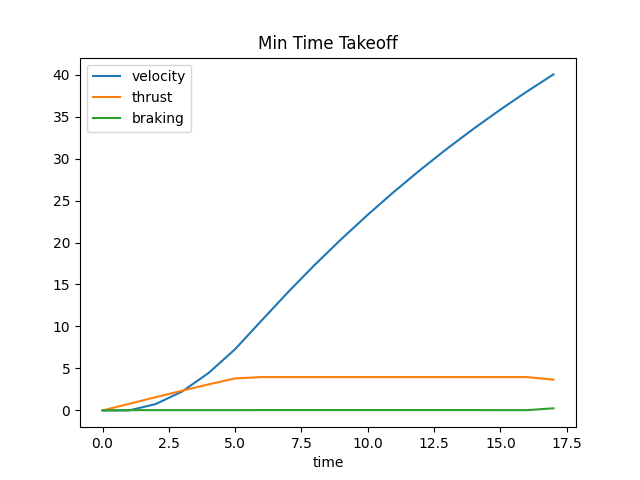
\includegraphics[scale=0.5]{p2_plot_no_position}
    \end{center}
    
    \begin{center}
    	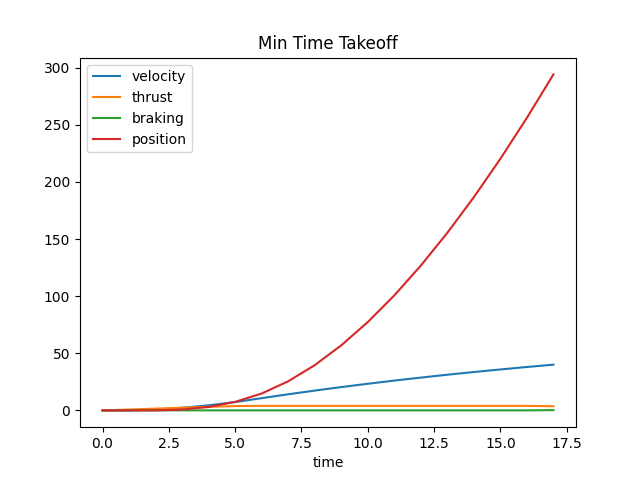
\includegraphics[scale=0.5]{p2_plot}
    \end{center}
    
\item (House profit and imputed probabilities) A set of $n$ participants bet on which of $m$ outcomes, labeled $1, \dots, m$, will occur. Participant $i$ offers to purchase up to $q_i > 0$ gambling contracts, at price $p_i > 0$, that the true outcome will be in the set $S_i \subset \{1, \dots, m\}$. The house then sells her $x_i$ contracts, with $0 \leq x_i \leq q_i$. If the true outcome $j$ is in $S_i$, then participant $i$ reeives \$1 per contract, i.e. $x_i$. Otherwise, she loses and receives nothing. The house collects a total of $x_1p_1 + \cdots + x_np_n$ and pays out an amount that depends on the outcome $j$, \[
        \sum_{i : j \in S_i} x_i.
    \] The difference is house profit.
    \begin{enumerate}
        \item How should the house decide on $x$ to maximize its worst case profit? We formulate the problem as a linear program. Immediately \[
            \sum_{i : j \in S_i} x_i
        \] is not clearly linear or convex, nor is optimizing over a discrete set $j \in \{1, \dots, m\}$. We reformulate the problem by introducing some new variables. First, call the above sum $t$, which is a number depending on the outcome $j$. Next, we organize the $S_i$ into one $m \times n$ matrix $S$ with \[
            S_{ji} = \begin{cases}
                1 & j \in S_i, \\
                0 & j \notin S_i.
            \end{cases}
        \] The problem becomes to maximize $p^T x - t$ such that $x \geq 0$, $x \leq q$, and $Sx \leq t$. Here when we write $\leq t$ we mean that every entry of $Sx$ is $\leq t$. Ideally we would set $Sx = t$, but $t$ is not affine so instead we equivalently say $Sx \leq t$, which is the same because the objective maximizes $-t$, so increasing it is detrimental. Now we would like to collapse $p^T x - t$ into a single dot product. We define \begin{align*}
            c &= \begin{bmatrix}
                p_1 & p_2 & \cdots & p_n & -1
            \end{bmatrix}^T, \\
            x' &= \begin{bmatrix}
                x_1 & x_2 & \cdots & x_n & t
            \end{bmatrix}^T.
        \end{align*} Now the objective becomes to minimize $c^T x'$. We collapse the constraints into a single matrix multiplication by defining the $(m + n) \times (n + 1)$ matrix \[
            A = \begin{bmatrix}
                I_n & 0 \\
                S & -1
            \end{bmatrix},
        \] where $I_n$ is the $n \times n$ identity matrix, $S$ is stacked underneath it and is $m \times n$, and we pad on the right with a single column of $n$ zeros to the right of $I_n$ and $m$ negative ones to the right of $S$. Define \[
            b = \begin{bmatrix}
                q_1 & \cdots & q_n & 0 & \cdots & 0
            \end{bmatrix}^T
        \] to be $n + m \times 1$. Our constraint is \[
            Ax' \leq b,
        \] along with $x' \geq 0$. The first $n$ rows of the inequality account for the constraints $x_i \leq q_i$, while the final $m$ rows account for the constraints \[
            t \geq \sum_{i : j \in S_i} x_i,
        \] running over each possible $j$, and ensuring that $t$ is greater than the maximum possible amount the house would need to pay out. Now an optimal $x^\ast$ for this linear program is one which minimizes worst case house profits, as desired.
    \end{enumerate}

    \item problem 4
\end{enumerate}

\end{document}
